%
% dimensionslos.tex
%
% (c) 2018 Prof Dr Andreas Müller, Hochschule Rapperswil
%
\section{Dynamik der thermohalinen Zirkulation}
\rhead{Dynamik der thermohalinen Zirkulation}
In diesem Abschnitt wollen wir die
Bewegungsgleichung~\ref{skript:thc:differenzgleichungen}
etwas vereinfachen mit dem Ziel, einzelne Szenarien durchspielen
zu können.
Eine vertiefte Diskussion solcher Modelle ist in
Kapitel~\ref{chapter:thermohalin} zu finden.

\subsection{Elimination von Prozessen mit kurzer Zeitkonstante}
Die Diskussion in Abschnitt~\ref{skript:thc:zeitkonstanten}
ist es zulässig, Variablen mit sehr kleiner Zeitkonstanten
durch Konstanten zu ersetzen.
Tatsächlich erfolgt der Temperaturausgleich im Wasser sehr viel
schneller als der Salinitätsausgleich.
Wir können daher davon ausgehen, dass die Temperaturgleichungen
die Temperaturanomalien sehr schnell gegen eine Gleichgewichtstemperatur
streben lassen und dass wir für die Lösung der Salinitätsgleichungen
mit dieser konstanten Temperatur arbeiten können.

Wir gehen also davon aus, dass $\Delta\bar T=2T^*$ konstant ist und
reduzieren damit das Gleichungssystem
\eqref{skript:thc:differenzgleichungen}
auf die eine Gleichung
\begin{equation}
\frac{d}{dt}\Delta\bar S
=
2H + d(2S^* -\Delta\bar S) - 2|q|\Delta\bar S
\qquad\text{mit}\qquad
q=k(2\alpha T^* -\beta \Delta\bar S).
\label{skript:thc:salinitaetallein}
\end{equation}
Diese Gleichungen beschreiben also die Salinitätsentwicklung unter
der Annahme, dass der Temperaturausgleich sehr schnell erfolgt.
Dieser Ausgleich kann nicht primär durch Durchmischung erfolgen,
denn dieser Mechanimus würde auch die Salinität mit gleicher
vergleichbarer Geschwindigkeit ausgleichen.
Dies bedeutet, dass der dominante Term in der Temperaturgleichung
der Term mit $c$ ist, nicht der Term mit $q$.

Die Gleichung \eqref{skript:thc:salinitaetallein} kann noch nicht auf
einfache Weise gelöst werden.
Wir vereinfachen wir sie daher weiter indem wir ausnutzen, dass 
der Salinitätsausgleich so viel langsamer ist als der Temperaturausgleich,
dass der Term mit $d$ im Vergleich zum Term mit $q$ vernachlässigbar ist.
Wir setzen also $d=0$ und
erhalten damit 
\begin{equation}
\frac{d}{dt}\Delta\bar S
=
2H - 2|q|\Delta\bar S
\qquad\text{mit}\qquad
q=k(2\alpha T^* -\beta \Delta\bar S)
\label{skript:thc:qgleichung}
\end{equation}
als vereinfachte Differentialgleichung zur Modellierung der 
thermohalinen Zirkulation.
Dies ist eine nichtlineare Differentialgleichung erster Ordnung,
die nicht in geschlossener Form gelöst werden kann.

\subsection{Eine dimensionslose Beschreibung}
Die Gleichung \eqref{skript:thc:qgleichung} ist wegen der vielen
Konstanten unübersichtlich.
Ausgeschrieben lautet sie
\begin{equation}
\frac{d}{dt}\Delta\bar S
=
2H
-2k|\alpha\Delta\bar T- \beta \Delta\bar S|\,\Delta\bar S
\label{skript:thc:smitdim}
\end{equation}
Die meisten der Konstanten können wir aber los werden, indem wir 
die unabhängigen Variablen und die Zeit neu skalieren.
Dies ist gleichbedeutend mit einem Wechsel der Masseinheiten.
Wir verwenden:
\begin{equation}
x=\frac{\beta\Delta\bar S}{\alpha\Delta\bar T},
\qquad
\tau = 2\alpha k\,|\Delta\bar T|\, t
\qquad\text{und}\qquad
\lambda = \frac{\beta H}{\alpha^2 k\Delta\bar T|\Delta\bar T|}.
\label{skript:thc:masseinheiten}
\end{equation}
Die Ableitung nach $t$ kann durch die Ableitung nach $\tau$ ausgedrücket
werden vermöge der Ersetzung
\[
\frac{d}{d\tau}
=
\frac{1}{2\alpha k|\Delta\bar T|}
\frac{d}{dt}
\qquad\Rightarrow\qquad
\frac{d}{dt}
=
2\alpha k|\Delta\bar T|\frac{d}{d\tau}.
\]
Setzen wir dies in die Gleichung~\eqref{skript:thc:masseinheiten}
ein, erhalten wir
\begin{equation}
2\alpha k|\Delta\bar T|
\frac{d}{d\tau} \Delta\bar S
=
2H-2k|\alpha\Delta\bar T-\beta\Delta\bar S|\,\Delta\bar S.
\end{equation}
Wir erweitern mit $\beta/\alpha\Delta\bar T$, damit wird die
Differentialgleichung zu
\begin{align}
2\alpha k|\Delta\bar T|
\frac{d}{d\tau}\frac{\beta\Delta\bar S}{\alpha\Delta\bar T}
&=
\frac{2\beta H}{\alpha\Delta\bar T} - 2k|\alpha\Delta\bar T-\beta\Delta\bar S|\,
\frac{\beta\Delta\bar S}{\alpha\Delta\bar T}
\notag
\\
\alpha k|\Delta\bar T|
\frac{d}{d\tau}x
&=
\frac{\beta H}{\alpha\Delta\bar T}
-k|\alpha\Delta\bar T-\beta\Delta\bar S|\, x
\notag
\\
k
\frac{d}{d\tau}x
&=
\frac{\beta H}{\alpha^2\Delta\bar T\,|\Delta\bar T|}
-k\biggl|1-\frac{\beta\Delta\bar S}{\alpha\Delta\bar T}\biggr|\,x
\notag
\\
\frac{d}{d\tau}x
&=
\frac{\beta H}{k\alpha^2\Delta\bar T\,|\Delta\bar T|}
-\biggl|1-\frac{\beta\Delta\bar S}{\alpha\Delta\bar T}\biggr|\,x
\notag
\\
\frac{dx}{d\tau}
&=
\lambda - |1-x|x.
\label{skript:thc:dimensionslos}
\end{align}
Damit haben wir die ursprüngliche Gleichung
\eqref{skript:thc:smitdim}
in eine dimensionslose Gleichung mit dem einen Parameter $\lambda$
umgewandelt.
Das Verhalten der Lösung hängt vom Parameter $\lambda$ ab.

\subsection{Gleichgewicht}
Um das Verhalten der Lösungen von 
\eqref{skript:thc:dimensionslos}
besser zu verstehen, suchen wir zunächst nach Gleichgewichtslösungen.
Diese hängen nicht von der Zeit ab, es gilt also
\begin{equation}
\frac{dx}{d\tau}=0
\qquad\Rightarrow\qquad
\lambda-|1-x|x=0
\qquad\Rightarrow\qquad
|1-x|x
=
\lambda.
\label{skript:thc:lambdagl}
\end{equation}
\begin{figure}
\centering
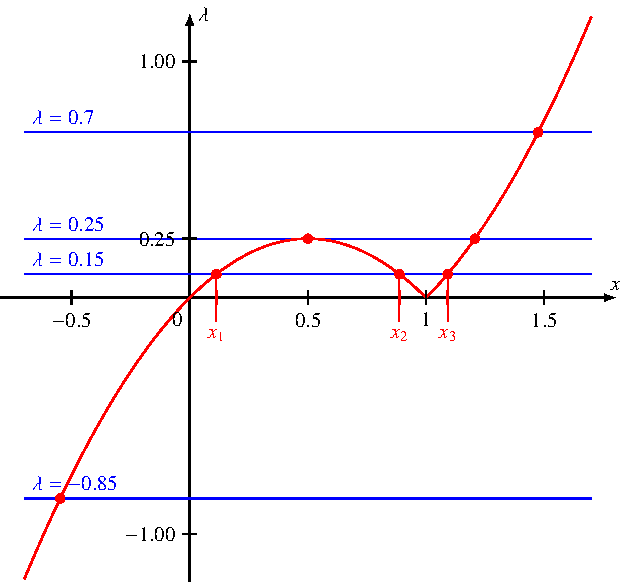
\includegraphics{chapters/4/rhs.pdf}
\caption{Graph der Funktion $|1-x|\,x$ und
Gleichgewichtslösungen der dimensionslosen Differentialgleichung
\eqref{skript:thc:dimensionslos}
\label{skript:thc:1-xxgraph}}
\end{figure}
In Abbildung~\ref{skript:thc:1-xxgraph} ist der Graph der Funktion 
$|1-x|\,x$ dargestellt.
Je nach dem Wert von $\lambda$ hat die dimensionslose Differentialgleichung
\eqref{skript:thc:dimensionslos} bis zu drei Gleichgewichtslösungen.

Für Werte von $\lambda$ zwischen $0$ und $0.25$ gibt es drei verschiedene
Werte $x$, die die Gleichung \eqref{skript:thc:lambdagl} erfüllen
(Abbildung~\ref{skript:thc:drei}).
Für $x\le 1$  ist $1-x\ge 0$ und damit muss $x$ die 
Gleichung $(1-x)x=\lambda$ erfüllen, für $x\ge 1$ ist es die Gleichung
$(x-1)x=\lambda$.
Diese beiden Gleichungen haben die folgenden Lösungen
\begin{align*}
&\text{Fall $x \le 1$:}
&
(1-x)x&=\lambda
&
&\text{Fall $x\ge 1$:}
&
(x-1)x&=\lambda
\\
&&
x^2-x+\lambda&=0
&&&
x^2-x-\lambda&=0
\\
&&
x&=\frac12\pm\sqrt{\frac14-\lambda}
&&&
x&=\frac12+\sqrt{\frac14+\lambda}.
\end{align*}
Die rechte Gleichung hat für alle Werte $\lambda > 0$ zwar auch noch
eine Lösung $<1$, diese ist aber ausgeschlossen, daher nur das
positive Zeichen vor der Wurzel in diesem Fall.
Für $\lambda > 0.25$ hat die linke Gleichung keine Lösung.
Für $\lambda < 0$ ist die Lösung mit dem positiven Zeichen der linken
Gleichung ausgeschlossen.

\begin{figure}
\centering
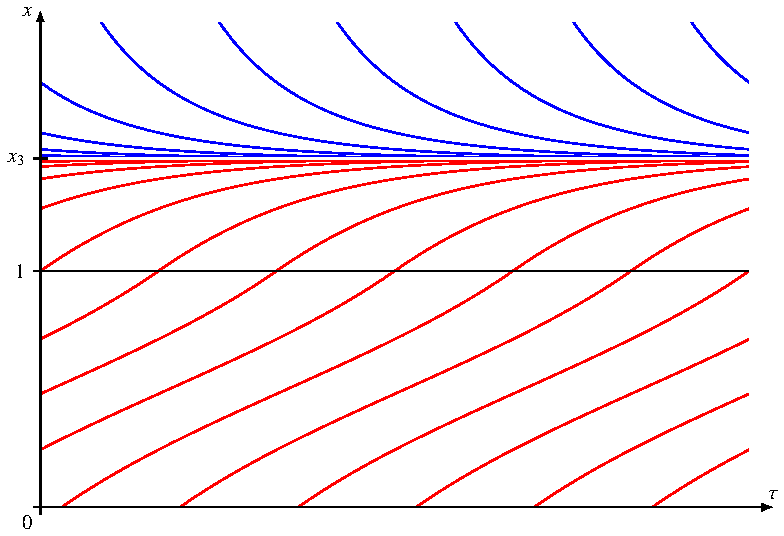
\includegraphics{chapters/4/ein.pdf}
\caption{Lösungen im Fall $\lambda > \frac14$: der einzige
Gleichgewichtspunkt $x_3$ ist stabil.
\label{skript:thc:ein}}
\end{figure}%
Wir berechnen die Lösung der Differentialgleichung für einen gegebenen
Wert von $\lambda$ (Abbildung~\ref{skript:thc:ein}).
Für $\lambda >\frac14$ gibt es nur einen Gleichgewichtspunkt, wir 
nennen ihn $x_3$.
Falls $x(\tau)<x_3$, dann ist
\[
\frac{dx}{d\tau}
=
\lambda - |1-x|x > 0,
\]
die Lösung $x(\tau)$ ist also monoton wachsend.
Für $x(\tau) > x_3$ ist hingegen
\[
\frac{dx}{d\tau}
=
\lambda - |1-x|x < 0,
\]
die Lösung ist also monoton wachsen.
Lösungskurven, die bei $x$-Werten $>x_3$ beginnen nehmen monoton ab
und konvergieren gegen $x_3$, solche, die bei $x$-Werten $<x_3$ beginnen,
nehmen monoton zu und konvergieren von unten gegen $x_3$.
Die Gleichgewichtslösung $x(\tau)=x_3$ ist also eine stabile Lösung,
alle anderen Lösungen konvergieren gegen diese Lösung.

\begin{figure}
\centering
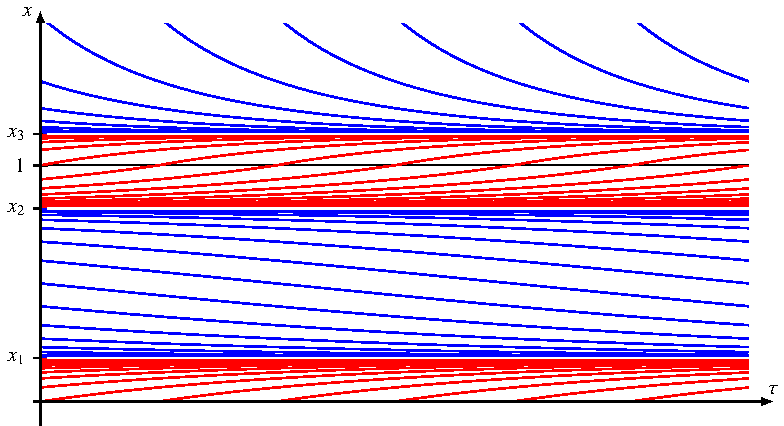
\includegraphics{chapters/4/drei.pdf}
\caption{Lösungen im Fall $0\le \lambda\le\frac14$: die beiden
Gleichgewichtspunkte $x_1$ und $x_3$ sind stabil, $x_2$ ist instabil.
\label{skript:thc:drei}}
\end{figure}%
Für $0<\lambda<\frac14$ seien
$x_1$, $x_2$ und $x_3$ die drei Gleichgewichtspunkte
(Abbildung~/ref{skript:thc:drei}).
Wir untersuchen wieder die Vorzeichen von $dx/d\tau$. 
Für $x$-Werten zwischen $x_1$ und $x_2$ und für $x$-Werte grösser
als $x_3$ ist die Ableitung positiv, die Lösungen konvergieren monoton
wachsend gegen die Gleichgewichtslösungen $x_1$ bzw.~$x_3$.
Lösungen, die bei $x<x_1$ oder $x_2<x<x_3$ beginnen, konvergieren
dagegen monoton wachsend gegen $x_1$ bzw.~$x_3$.
Die Gleichgewichtslösung $x_2$ ist daher nicht stabil,
die Gleichgewichtslösungen $x_1$ und $x_3$ sind dagegen stabil.

\subsection{Bifurkation}
\begin{figure}
\centering
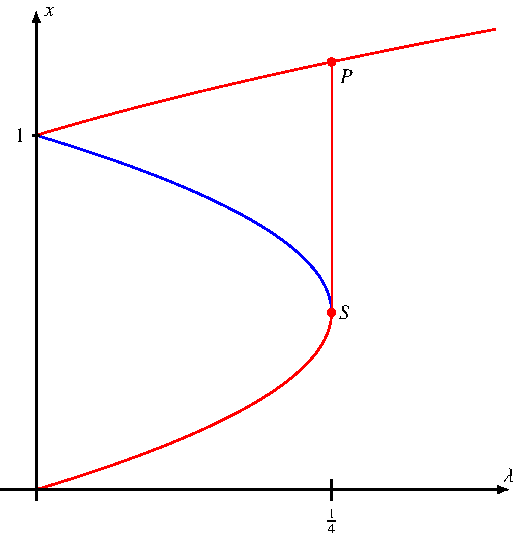
\includegraphics{chapters/4/bi.pdf}
\caption{Bifurkationsdiagramm für die Differentialgleichung
\eqref{skript:thc:lambdagl}
\label{skript:thc:bifurkation}}
\end{figure}
Für Parameterwerte $\lambda < \frac14$ gibt es drei mögliche
Gleichgewichtspunkte, für $\lambda>\frac14$ jedoch nur noch einen.
Wir möchten untersuchen, wie sich die Lösung verhält, wenn der
Parameter langsam verändert wird.
Dies ist in Abbildung~\ref{skript:thc:bifurkation} dargestellt.

Sei jetzt also zunächst $\lambda <\frac14$.
Wir betrachten also eine Lösung, die in Nähe von
\[
x_1(\lambda)=\frac12-\sqrt{\frac14-\lambda}
\]
beginnt.
Vergrössern wir $\lambda$, verschiebt sich der Gleichgewichtspunkt
$x_1(\lambda)$ ebenfalls nach oben.
Da $x_1(\lambda)$ aber ein stabiler Gleichgewichtspunkt ist, wird die
Lösung gegen den neuen Gleichgewichtspunkt konvergieren.
Das gleiche passiert auch, wenn die Lösung in der Nähe von
\[
x_3(\lambda)=\frac12+\sqrt{\frac14+\lambda}
\]
beginnt.
Bei einer Vergrösserung folgt das System den roten Kurven in
Abbildung~\ref{skript:thc:bifurkation}.

Wenn jetzt aber der Parameter $\lambda$ die Schwelle $\frac14$
überschreitet, dann wird die Lösung zum einzigen verbleibenden
stabilen Gleichgewichtspunkt $x_3(\lambda)$ konvergieren.
Die Lösung springt also vom Punkt $S$ zum Punkt $P$ auf dem oberen roten Ast
in Abbildung~\ref{skript:thc:bifurkation}.

Wenn man den Parameter $\lambda$ wieder verkleinert, dann wird
eine Lösung in der Nähe von $x_3(\lambda)$ wieder gegen
$x_3(\lambda)$ konvergieren.
Es ist aber nicht mehr möglich, dass die Lösung gegen $x_1(\lambda)$
konvergiert, da nach Abbildung~\ref{skript:thc:drei} nur Lösungen,
die bei $x$-Werten $<x_2$ beginnen, gegen $x_1(\lambda)$ konvergieren
können.

Dieses einfache Modell der thermohalinen Zirkulation hat also die
überraschende Eigenschaft, dass das System beim Überschreiten des
kritischen Wertes $\lambda=\frac14$ in einen Zustand kippt, aus dem
es nicht mehr zurück kommen kann.
Wegen
\[
\lambda
=
\frac{\beta H}{\alpha^2k\Delta\bar T\,|\Delta\bar T|}
\]
kann dies passieren wenn entweder der Betrag des virtuellen Salzflusses 
$H$ ansteigt oder die Temperaturanomaliedifferenz $\Delta\bar T$
klein wird.
Eine Klimaerwärmung könnte zum Beispiel die Verdunstung im Gebiet $2$
erhöhen, den virtuellen Salzfluss erhöhen und damit das System
in den Zustand mit einer wesentlich grösseren Anomaliedifferenz
$\Delta\bar S$ kippen lassen.





